\chapter{Áp suất, năng lượng tự do và thăng giáng năng lượng}

\lectureoverview{Ta suy ra áp suất từ hàm phân hoạch mà không giả định một bức tranh động học trong đó các phân tử va vào thành. Một bổ đề hình học chuyển một đạo hàm đoạn nhiệt thành các đạo hàm ở nhiệt độ cố định, năng lượng tự do Helmholtz làm cầu nối tới \(\log Z\), và định luật khí lý tưởng xuất hiện như ứng dụng đầu tiên. Sau đó ta dùng cùng hàm phân hoạch ấy để suy ra thăng giáng năng lượng cân bằng và quan hệ của nó với nhiệt dung.}

\section{Để toán học kiểm nghiệm trực giác}

Nhiệt động lực học có một danh tiếng khá đặc biệt. Phép tính của nó là sơ cấp, nhưng việc chọn lấy đạo hàm theo đại lượng nào và giữ cố định đại lượng nào có thể tinh tế đến mức đáng ngạc nhiên. Bài toán của ta được cố ý thu hẹp: tính áp suất của một khí lý tưởng. Tuy nhiên, con đường đi tới câu trả lời ấy được chủ ý làm đủ tổng quát cho những hệ trong đó bức tranh phân tử quen thuộc không còn đáng tin cậy nữa.

Câu chuyện động học thì dễ kể. Các phân tử va vào một bức tường và đảo dấu thành phần pháp tuyến của động lượng của chúng. Động lượng truyền trong một đơn vị thời gian cho ta lực, và lực trên một đơn vị diện tích cho ta áp suất. Ta đã biết rằng động năng trung bình trên mỗi phân tử trong ba chiều là
\begin{equation}
 \left\langle \frac{p^2}{2m}\right\rangle=\frac{3}{2}T
 \qquad (k_B=1).
 \label{eq:sm5-mean-kinetic-energy}
\end{equation}
Với một phân bố vận tốc đẳng hướng, ta có thể ước lượng tốc độ va chạm, độ truyền động lượng trong mỗi va chạm, và áp suất thu được.

Nhưng chính bức tường dường như lại phá vỡ tính đẳng hướng. Vì sao các phân tử rất gần biên lại phải có cùng phân bố về tốc độ và hướng như các phân tử ở sâu trong lòng hệ? Ở cân bằng thì đúng là như vậy, với độ chính xác thích hợp ở đây, nhưng kết luận ấy phải được suy ra từ cơ học thống kê chứ không nên bị lén đưa vào phép tính dưới dạng trực giác. Các va chạm giữa các phân tử còn khiến lập luận động học kém minh bạch hơn nữa. Khí không tương tác là dễ chính vì nó là một hệ đơn giản một cách khác thường.

Trong vật lý có những lúc thủ tục an toàn nhất là tạm thời gác bức tranh trực quan sang một bên và đi theo toán học. Ta xác định đại lượng cần tìm, thao tác các quan hệ tổng quát, rồi chờ cho tới khi xuất hiện một công thức dễ nhận ra. Trực giác quay trở lại ở cuối, nhưng khi đó toán học đang kiểm nghiệm trực giác chứ không phải ngược lại. Cái thú của nhiệt động lực học nằm ở những quan hệ bất ngờ nảy sinh từ thủ tục này.

Quan hệ ta cần là một phương trình trạng thái,
\begin{equation}
 P=P(T,V,N),
 \label{eq:sm5-equation-of-state-target}
\end{equation}
trong đó \(N\) là lượng vật chất, \(T\) là nhiệt độ và \(V\) là thể tích. Một phép suy dẫn thỏa đáng vẫn phải có nghĩa khi các hạt tương tác, hoặc khi vật chất là chất lỏng, plasma hay chất rắn. Chỉ việc đánh giá cuối cùng của hàm phân hoạch mới chuyên biệt cho khí lý tưởng.

\section{Entropy và năng lượng tự do Helmholtz}

Hãy bắt đầu bằng cách nhắc lại các công thức chính tắc sẽ cần đến về sau. Với các vi trạng thái được gắn nhãn bởi \(i\),
\begin{equation}
 \begin{aligned}
 S&=-\sum_i p_i\log p_i,\\
 p_i&=\frac{e^{-\beta E_i}}{Z},\\
 Z&=\sum_i e^{-\beta E_i}.
 \end{aligned}
 \label{eq:sm5-canonical-definitions}
\end{equation}
Logarit của xác suất là
\begin{equation}
 \log p_i=-\beta E_i-\log Z.
 \label{eq:sm5-log-probability}
\end{equation}
Thế vào entropy, ta được
\begin{align}
 S
 &=-\sum_i p_i\log p_i \notag\\
 &=\beta\sum_i p_iE_i+\log Z\sum_i p_i \notag\\
 &=\beta E+\log Z.
 \label{eq:sm5-entropy-log-z}
\end{align}
Ở đây \(E=\sum_i p_iE_i\) là năng lượng trung bình.

\begin{classroomqa}
\audiencequestion{Vì sao hạng thứ hai chỉ cho \(\log Z\), chứ không phải số trạng thái nhân với \(\log Z\)?}
\lecturerresponse{Hệ số đang được lấy tổng là \(p_i\), không phải \(1\).
Điều kiện chuẩn hóa cho \(\sum_i p_i=1\). Tương đương, tử số
\(\sum_i e^{-\beta E_i}=Z\) triệt tiêu \(Z\) ở mẫu. Số trạng thái không bao giờ xuất hiện ở bước này.
\lecturetimestamp{00:14:25--00:14:55}}
\end{classroomqa}

Trong các đơn vị năng lượng được dùng trong phần lớn bài giảng,
\(\beta=1/T\). Nhân \eqref{eq:sm5-entropy-log-z} với \(T\) rồi sắp xếp lại, ta được
\begin{equation}
 E-TS=-T\log Z.
 \label{eq:sm5-helmholtz-identity}
\end{equation}
Tổ hợp ở vế trái xuất hiện thường xuyên đến mức xứng đáng có một tên gọi:
\begin{equation}
 A\equiv E-TS,
 \qquad
 A=-T\log Z.
 \label{eq:sm5-helmholtz-definition}
\end{equation}
Đó là năng lượng tự do Helmholtz. Lúc này tên gọi kém quan trọng hơn chính đồng nhất thức ấy; ta sẽ cần đồng nhất thức đó khi áp suất được chuyển thành một đạo hàm của hàm phân hoạch.

\begin{figure}[t]
\centering
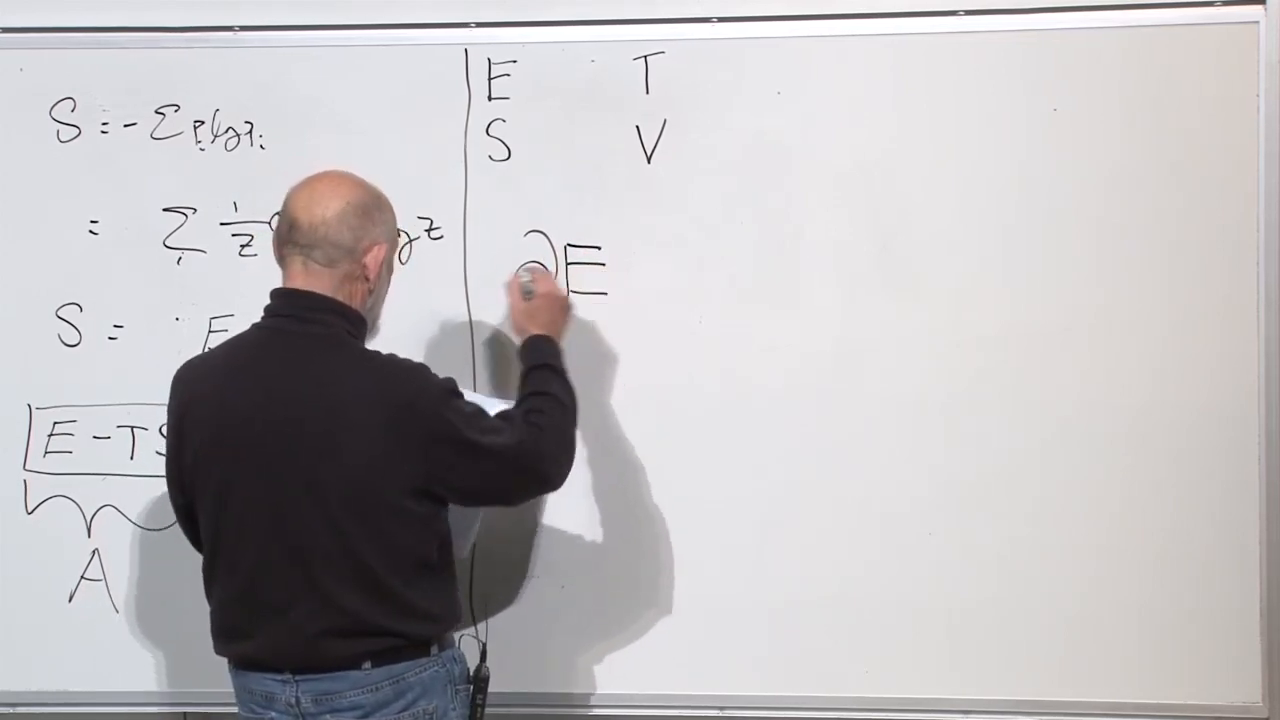
\includegraphics[width=0.90\textwidth]{lecture_05_figure_03.png}
\caption{Quan hệ entropy chính tắc được viết lại thành
\(A=E-TS=-T\log Z\).}
\lectureframe{00:16:50}
\end{figure}

\section{Các tham số điều khiển và các đáp ứng của chúng}

Một tham số điều khiển là một đại lượng vĩ mô mà nhà thực nghiệm có thể thay đổi từ bên ngoài. Di chuyển một pít-tông làm thay đổi thể tích mà không cần thao tác lên từng phân tử riêng lẻ. Điện trường và từ trường áp đặt từ bên ngoài là những ví dụ khác. Trong một quần thể thống kê tổng quát hơn, số hạt cũng có thể được phép thay đổi.

Các biến nhiệt động tự nhiên đi thành những cặp liên hợp. Trong bài toán hiện tại, thể tích là tham số điều khiển và áp suất là đáp ứng của nó. Ta thay đổi \(V\); áp suất cho ta biết hệ chống lại sự thay đổi ấy về mặt năng lượng như thế nào. Về sau, đạo hàm của năng lượng sẽ làm cho sự ghép cặp này trở nên chính xác.

\begin{classroomqa}
\audiencequestion{Bản thân áp suất có thể được xem là tham số điều khiển không?}
\lecturerresponse{Ta có thể thiết kế một thí nghiệm cố định áp suất ngoài, nhưng trong cách dựng dùng ở đây, vị trí pít-tông cố định thể tích và áp suất bên trong là đáp ứng. Áp suất và thể tích là các biến liên hợp; thành phần nào được điều khiển còn tùy vào quần thể và thiết bị.
\lecturetimestamp{00:19:22--00:20:01}}
\end{classroomqa}

\begin{classroomqa}
\audiencequestion{Có phải mọi phân tử đều được giả sử là đồng nhất, hay lập luận này chỉ giới hạn cho chất khí?}
\lecturerresponse{Không cần sự hạn chế nào như vậy cho lập luận nhiệt động. Xi lanh có thể chứa nhiều loại hạt, một chất lỏng, hoặc thậm chí một chất rắn đang bị nén. Hàm phân hoạch của khí lý tưởng sẽ chỉ là một áp dụng riêng sau khi công thức áp suất tổng quát đã được thiết lập.
\lecturetimestamp{00:20:02--00:20:39}}
\end{classroomqa}

\begin{classroomqa}
\audiencequestion{Lượng vật chất có thể được thay đổi như một thao tác ngoài khác không?}
\lecturerresponse{Có. Số hạt là một tham số điều khiển khả dĩ khác. Khi xét nó như một biến có thể thay đổi, ta đi tới đại lượng liên hợp riêng của nó, là thế hóa học. Trong phép tính tối nay, \(N\) được giữ cố định.
\lecturetimestamp{00:20:39--00:20:57}}
\end{classroomqa}

\begin{classroomqa}
\audiencequestion{Nước lỏng và hơi nước có thể hiện diện đồng thời trong cân bằng không?}
\lecturerresponse{Ở nhiệt độ và áp suất đồng tồn tại thì có thể. Trọng lực có thể đặt phần lỏng ở dưới phần hơi, nhưng hai pha vẫn có thể có cùng một nhiệt độ và duy trì cân bằng nhiệt. Cùng một khuôn khổ cơ học thống kê tổng quát vẫn áp dụng được.
\lecturetimestamp{00:20:59--00:21:36}}
\end{classroomqa}

Trong lập luận tiếp theo, hãy coi năng lượng và entropy là các hàm phụ thuộc của hai biến có thể điều chỉnh độc lập:
\begin{equation}
 E=E(T,V),
 \qquad
 S=S(T,V).
 \label{eq:sm5-dependent-functions}
\end{equation}
Nhiệt độ và thể tích cung cấp các tọa độ trên một không gian trạng thái nhiệt động. Năng lượng và entropy gán các giá trị số cho mọi điểm cân bằng trong không gian ấy.

\section{Đạo hàm ở entropy không đổi}

Đạo hàm cuối cùng ta cần đến là một đạo hàm khác thường:
\[
 \left(\frac{\partial E}{\partial V}\right)_S.
\]
Mặc dù \(T\) và \(V\) là các tọa độ độc lập, đạo hàm này yêu cầu ta thay đổi \(V\) đồng thời ràng buộc hàm phụ thuộc \(S(T,V)\) giữ không đổi. Đó là một đạo hàm dọc theo một đường cong trong mặt phẳng \((T,V)\), chứ không phải dọc theo một trục tọa độ.

\begin{classroomqa}
\audiencequestion{Làm sao \(T\) và \(V\) có thể độc lập nếu về sau lại dùng đạo hàm \(dT/dV\)?}
\lecturerresponse{Chúng độc lập trên toàn bộ không gian trạng thái. Một khi ta áp đặt ràng buộc \(S(T,V)=\mathrm{constant}\), các trạng thái được phép sẽ nằm trên một đường cong một chiều. Dọc theo đường đó, \(T\) trở thành một hàm của \(V\), và độ dốc của nó \(dT/dV\) được xác định rõ.
\lecturetimestamp{01:01:18--01:02:09}}
\end{classroomqa}

\begin{lemma}
Nếu \(E(T,V)\) và \(S(T,V)\) khả vi, thì ở mọi nơi mà
\((\partial S/\partial T)_V\neq0\),
\begin{equation}
 \left(\frac{\partial E}{\partial V}\right)_S
 =
 \left(\frac{\partial E}{\partial V}\right)_T
 -
 \left(\frac{\partial E}{\partial S}\right)_V
 \left(\frac{\partial S}{\partial V}\right)_T.
 \label{eq:sm5-calculus-lemma}
\end{equation}
\end{lemma}

\begin{proof}
Với một dịch chuyển vi phân bất kỳ,
\begin{equation}
 dE=
 \left(\frac{\partial E}{\partial V}\right)_T dV
 +
 \left(\frac{\partial E}{\partial T}\right)_V dT.
 \label{eq:sm5-total-differential-e}
\end{equation}
Khi giữ cố định \(V\), quy tắc dây chuyền cho phép dùng \(S\) làm biến trung gian:
\begin{equation}
 \left(\frac{\partial E}{\partial T}\right)_V
 =
 \left(\frac{\partial E}{\partial S}\right)_V
 \left(\frac{\partial S}{\partial T}\right)_V.
 \label{eq:sm5-chain-rule-e-s-t}
\end{equation}

Bây giờ hãy giới hạn dịch chuyển vào một đường cong mà trên đó \(S\) không đổi.
Dọc theo đường đó,
\begin{equation}
 0=dS=
 \left(\frac{\partial S}{\partial V}\right)_T dV
 +
 \left(\frac{\partial S}{\partial T}\right)_V dT.
 \label{eq:sm5-constant-entropy-differential}
\end{equation}
Giải theo độ dốc của đường cong, ta được
\begin{equation}
 \left(\frac{dT}{dV}\right)_S
 =
 -
 \frac{\left(\frac{\partial S}{\partial V}\right)_T}
 {\left(\frac{\partial S}{\partial T}\right)_V}.
 \label{eq:sm5-entropy-contour-slope}
\end{equation}
Chia \eqref{eq:sm5-total-differential-e} cho \(dV\), dùng
\eqref{eq:sm5-chain-rule-e-s-t}, rồi thế
\eqref{eq:sm5-entropy-contour-slope} vào:
\begin{align}
 \left(\frac{\partial E}{\partial V}\right)_S
 &=
 \left(\frac{\partial E}{\partial V}\right)_T
 +
 \left(\frac{\partial E}{\partial S}\right)_V
 \left(\frac{\partial S}{\partial T}\right)_V
 \left(\frac{dT}{dV}\right)_S \notag\\
 &=
 \left(\frac{\partial E}{\partial V}\right)_T
 -
 \left(\frac{\partial E}{\partial S}\right)_V
 \left(\frac{\partial S}{\partial V}\right)_T.
\end{align}
Thừa số \((\partial S/\partial T)_V\) đã triệt tiêu, qua đó chứng minh kết quả.
\end{proof}

\begin{figure}[t]
\centering
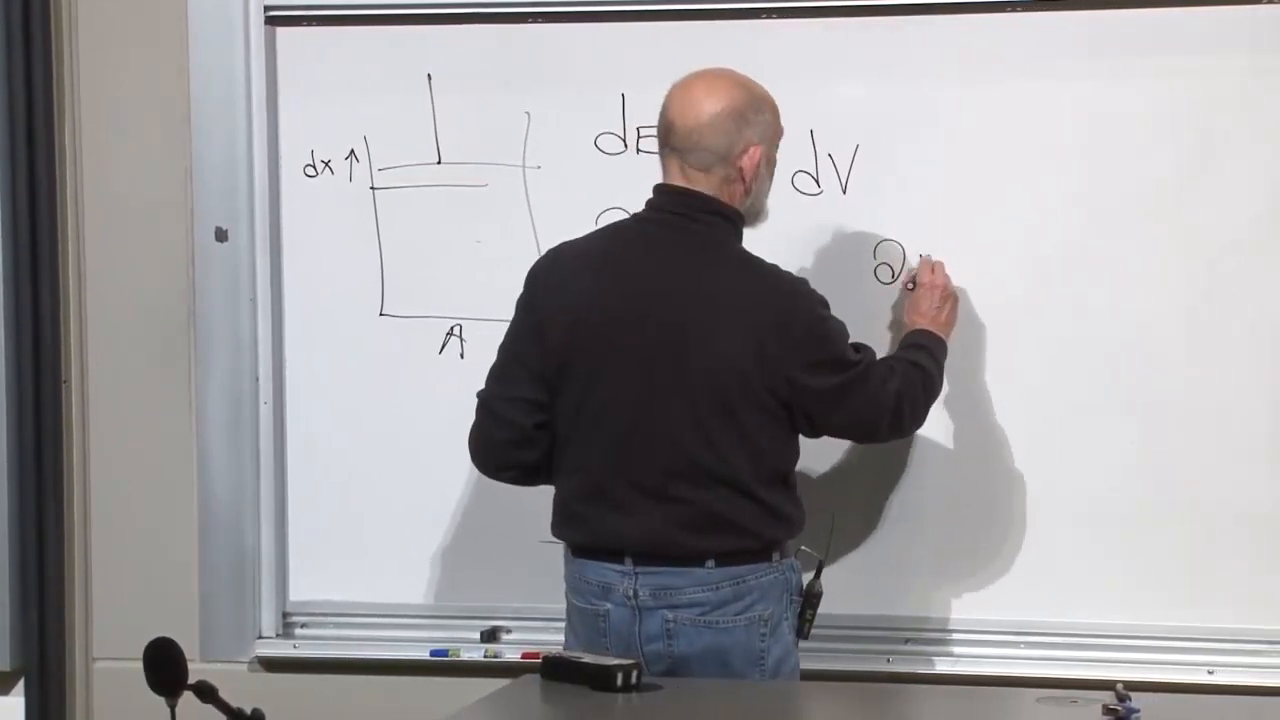
\includegraphics[width=0.90\textwidth]{lecture_05_figure_04.png}
\caption{Phép tính trên đường mức entropy không đổi tại bước triệt tiêu, bước hoàn tất bổ đề về đạo hàm.}
\lectureframe{00:36:10}
\end{figure}

Bức tranh hình học không phải chỉ để trang trí. Nó giải thích vì sao một đạo hàm có vẻ lạ ở \(S\) không đổi có thể được tính bằng các đạo hàm riêng thông thường theo các tọa độ độc lập \(T\) và \(V\). Việc viết \(\delta E/\delta V\) trong quá trình xây dựng là một lời nhắc hữu ích rằng các ký hiệu ấy biểu diễn những tỉ số của các biến thiên nhỏ dọc theo một đường đi đã được chỉ rõ.

\begin{classroomqa}
\audiencequestion{Khai triển của \(dE\) có phải chỉ là định nghĩa thông thường của các đạo hàm riêng không?}
\lecturerresponse{Có. Không có gì đặc biệt xảy ra trong vi phân toàn phần. Yếu tố thêm vào duy nhất là sự hạn chế về sau vào đường cong \(dS=0\), vốn xác định quan hệ giữa \(dT\) và \(dV\).
\lecturetimestamp{00:29:26--00:29:32}}
\end{classroomqa}

\begin{classroomqa}
\audiencequestion{Có phải để triệt tiêu được thì
\((\partial S/\partial T)_V\) phải khác không?}
\lecturerresponse{Có. Đối với một hệ ổn định thông thường,
\[
 \left(\frac{\partial S}{\partial T}\right)_V
 =\frac{C_V}{T}>0,
\]
nên phép chia là hợp lệ. Những điểm ngoại lệ đòi hỏi phải được xét riêng.
Khi Hamiltonian được giữ cố định, tăng nhiệt độ làm phân bố năng lượng chính tắc rộng ra và thông thường làm entropy tăng; hạ nhiệt độ làm nó hẹp lại. Đây là hướng đúng về mặt vật lý của lập luận về tính đơn điệu.
\lecturetimestamp{00:36:50--00:37:47}}
\end{classroomqa}

\section{Công của pít-tông và điều kiện đoạn nhiệt}

Bây giờ ta gán cho đạo hàm này một ý nghĩa vật lý. Hãy xét một pít-tông có
tiết diện ngang \(\mathcal A\). Nếu nó dịch ra ngoài một đoạn \(dx\), thì
\begin{equation}
 dV=\mathcal A\,dx.
 \label{eq:sm5-piston-volume}
\end{equation}
Khí tác dụng lực \(P\mathcal A\) lên pít-tông, nên công do khí thực hiện là
\begin{equation}
 \delta W_{\mathrm{by}}=P\mathcal A\,dx=P\,dV.
 \label{eq:sm5-piston-work}
\end{equation}
Nếu không có nhiệt đi vào khí, định luật bảo toàn năng lượng cho
\begin{equation}
 dE=-P\,dV.
 \label{eq:sm5-adiabatic-work}
\end{equation}
Dấu này có ý nghĩa vật lý: trong quá trình giãn nở, khí nâng pít-tông lên hoặc gia tốc cho nó, và năng lượng của chính khí giảm đi.

\begin{figure}[t]
\centering
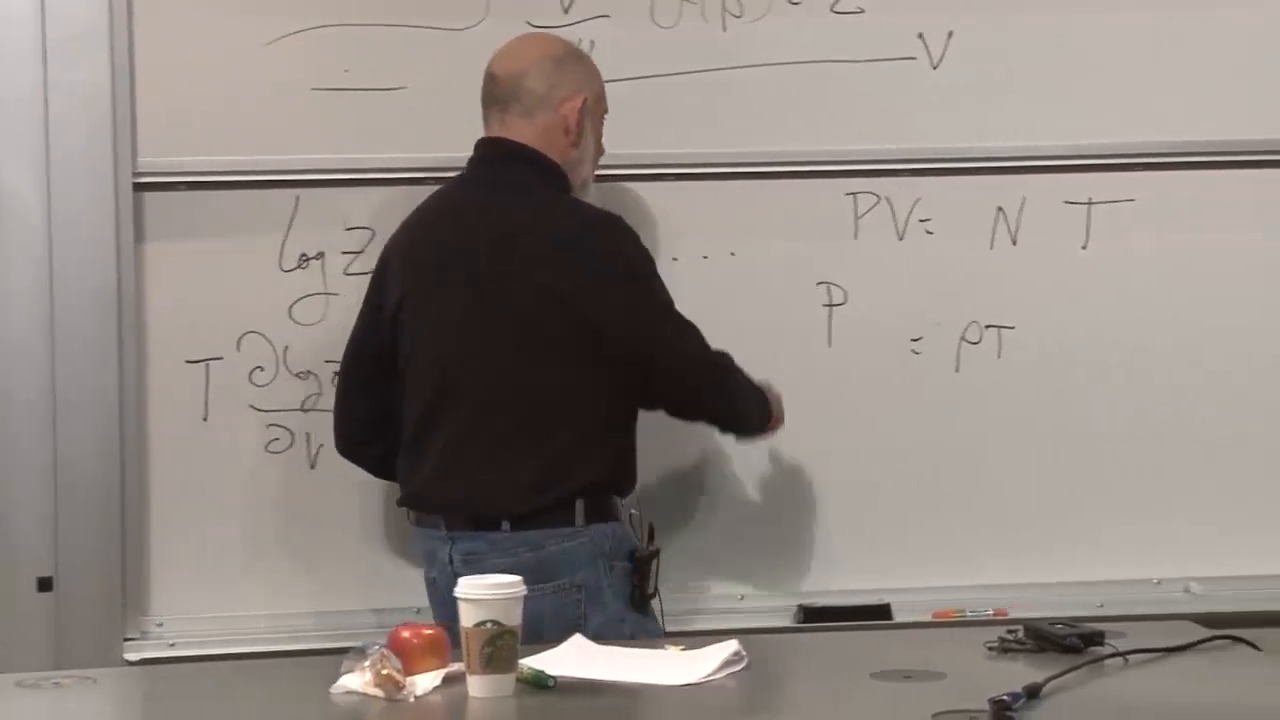
\includegraphics[width=0.90\textwidth]{lecture_05_figure_05.png}
\caption{Hình học của pít-tông và hệ thức công suy ra được
\(dE=-P\,dV\).}
\lectureframe{00:43:10}
\end{figure}

Hai lưu ý là thiết yếu. Pít-tông phải chuyển động đủ chậm để
hệ luôn ở gần cân bằng đến mức tùy ý, và thành bình phải được
cách nhiệt để năng lượng không được cung cấp dưới dạng nhiệt. Một sự kéo ra nhanh có thể
nhanh đến mức không phân tử nào chạm tới pít-tông đang lùi trong khi nó chuyển động. Một
sự nén nhanh tạo ra sóng xung kích. Không quá trình nào trong hai quá trình ấy được biểu diễn bằng
một dãy trạng thái cân bằng.

Từ \emph{đoạn nhiệt} đôi khi được dùng để chỉ không có truyền nhiệt và
đôi khi để chỉ biến đổi chậm. Trong quá trình thuận nghịch cần có ở đây, cả hai
ý đều tham gia: biến đổi là quasi-tĩnh và được cách nhiệt. Trong các điều
kiện đó, nó cũng là đẳng entropy.

\begin{classroomqa}
\audiencequestion{Vì sao một biến đổi đoạn nhiệt giữ entropy cố định?}
\lecturerresponse{Hãy nhìn hệ theo cơ học lượng tử. Các mức
năng lượng nhiều hạt của nó phụ thuộc vào thể tích. Khi \(V\) thay đổi chậm, định lý đoạn nhiệt
đưa mỗi mức đang bị chiếm liên tục sang mức tương ứng tiếp theo của nó mà không có
chuyển giữa các nhãn mức. Các năng lượng \(E_i(V)\) thay đổi, nhưng các
xác suất chiếm \(p_i\) vẫn giữ nguyên. Vì
\(S=-\sum_i p_i\log p_i\) phụ thuộc vào các xác suất đó, entropy vẫn
không đổi. Sự trao đổi nhiệt hoặc chuyển động không thuận nghịch sẽ làm kết luận
này không còn đúng.
\lecturetimestamp{00:43:37--00:49:15}}
\end{classroomqa}

\begin{figure}[t]
\centering
\includegraphics[width=0.90\textwidth]{lecture_05_figure_06.png}
\caption{Các mức năng lượng nhiều hạt biến thiên theo thể tích trong khi các
xác suất chiếm của chúng vẫn giữ nguyên các nhãn mức.}
\lectureframe{00:48:50}
\end{figure}

Phương trình \eqref{eq:sm5-adiabatic-work}, khi được đánh giá dọc theo đường
entropy không đổi này, xác định áp suất là
\begin{equation}
 P=-\left(\frac{\partial E}{\partial V}\right)_S.
 \label{eq:sm5-pressure-fixed-entropy}
\end{equation}
Đây là hệ thức liên hợp giữa áp suất và thể tích.

\begin{classroomqa}
\audiencequestion{Điều gì xảy ra nếu thay vào đó pít-tông được dịch chuyển nhanh?}
\lecturerresponse{Hệ rời khỏi cân bằng và động lực học chi tiết của nó
trở nên quan trọng. Nén đột ngột tạo ra một sóng xung kích. Trong một sự giãn nở tự do lý tưởng,
pít-tông có thể lùi đi trước khi bất kỳ phân tử nào va vào nó, nên không có công nào được thực hiện và
năng lượng vẫn giữ nguyên dù thể tích thay đổi. Về sau khí
thư giãn về cân bằng với entropy tăng lên. Những quá trình như vậy không thể được
mô tả bằng đạo hàm cân bằng duy nhất trong
\eqref{eq:sm5-pressure-fixed-entropy}.
\lecturetimestamp{00:58:30--01:01:15}}
\end{classroomqa}

\begin{classroomqa}
\audiencequestion{Điều kiện định lượng nào quyết định một biến đổi có
chậm hay không?}
\lecturerresponse{Thời gian biến thiên của tác động bên ngoài phải dài so với
các thời gian thư giãn nội tại liên quan. Đối với một chất khí, nhiều va chạm
phân tử và nhiều lần va vào thành phải xảy ra trong suốt biến đổi vĩ mô.
Thang thời gian chính xác phụ thuộc vào vật liệu và hình học, còn bản thân
giới hạn quasi-tĩnh thì là tổng quát.
\lecturetimestamp{01:02:09--01:03:20}}
\end{classroomqa}

\section{Từ năng lượng đoạn nhiệt đến hàm phân hoạch}

Công thức vật lý \eqref{eq:sm5-pressure-fixed-entropy} vẫn chưa phải là công thức
dễ tính. Cơ học thống kê chính tắc tự nhiên cung cấp
các hàm theo nhiệt độ, vì \(T\) xuất hiện trực tiếp trong
trọng số Boltzmann. Bổ đề giải tích chuyển đạo hàm ở entropy cố định, vốn bất tiện,
sang ngôn ngữ tính toán đó:
\begin{align}
 P
 &=
 -\left(\frac{\partial E}{\partial V}\right)_T
 +
 \left(\frac{\partial E}{\partial S}\right)_V
 \left(\frac{\partial S}{\partial V}\right)_T.
 \label{eq:sm5-pressure-lemma-substitution}
\end{align}
Ở thể tích cố định, định luật một cho \(dE=T\,dS\), và do đó
\begin{equation}
 \left(\frac{\partial E}{\partial S}\right)_V=T.
 \label{eq:sm5-e-s-temperature}
\end{equation}
Vì vậy
\begin{equation}
 P=
 -\left(\frac{\partial E}{\partial V}\right)_T
 +
 T\left(\frac{\partial S}{\partial V}\right)_T.
 \label{eq:sm5-pressure-fixed-temperature-pieces}
\end{equation}

\begin{classroomqa}
\audiencequestion{Dấu trừ trong công thức áp suất bắt nguồn từ
đâu?}
\lecturerresponse{Nó bắt nguồn từ công do khí thực hiện:
\(dE=-P\,dV\) trong giãn nở đoạn nhiệt. Bản thân bổ đề giải tích có một
dấu trừ giữa hai hạng của nó; dấu trừ toàn cục trong
\(P=-(\partial E/\partial V)_S\) đảo dấu của cả hai hạng ấy, cho ra
\eqref{eq:sm5-pressure-fixed-temperature-pieces}.
\lecturetimestamp{00:52:40--00:53:14}}
\end{classroomqa}

Bởi vì \(T\) được giữ cố định trong cả hai đạo hàm,
\begin{align}
 P
 &=
 -\left(\frac{\partial}{\partial V}(E-TS)\right)_T \notag\\
 &=
 -\left(\frac{\partial A}{\partial V}\right)_T.
 \label{eq:sm5-pressure-free-energy}
\end{align}
Cuối cùng thay \(A=-T\log Z\) vào:
\begin{equation}
 \boxed{
 P=
 T\left(\frac{\partial\log Z}{\partial V}\right)_T
 }.
 \label{eq:sm5-pressure-log-z}
\end{equation}

\begin{figure}[t]
\centering
\includegraphics[width=0.90\textwidth]{lecture_05_figure_07.png}
\caption{Phiên bản cô đọng ở nhiệt độ cố định của lập luận:
\(P=-(\partial A/\partial V)_T
=T(\partial\log Z/\partial V)_T\).}
\lectureframe{00:55:55}
\end{figure}

Không có gì trong \eqref{eq:sm5-pressure-log-z} giả sử khí lý tưởng. Nếu có thể
tính được hàm phân hoạch cho một chất lưu tương tác, plasma hoặc
chất rắn, thì cùng đạo hàm đó cho áp suất của nó. Tổng quát hơn, mọi
tham số điều khiển bên ngoài đều có một đáp ứng liên hợp thu được bằng cách
lấy đạo hàm của một thế nhiệt động thích hợp. Hàm phân hoạch
mã hóa nhiều đáp ứng như vậy: lấy đạo hàm \(\log Z\) theo
\(\beta\) cho năng lượng, còn lấy đạo hàm của nó theo
thể tích cho áp suất.

\section{Phương trình trạng thái của khí lý tưởng}

Chỉ đến lúc này ta mới chuyên biệt hóa sang \(N\) hạt không tương tác. Vẫn giữ nguyên
chuẩn hóa không gian pha cổ điển,
\begin{equation}
 Z_N=
 \frac{1}{N!h^{3N}}
 \int d^{3N}q\,d^{3N}p\,
 \exp\!\left[
 -\beta\sum_{a=1}^{N}\frac{\mathbf p_a^2}{2m}
 \right].
 \label{eq:sm5-ideal-gas-partition-integral}
\end{equation}
Có \(3N\) tọa độ vị trí và \(3N\) tọa độ động lượng. Hamiltonian
không phụ thuộc vào vị trí, nên mỗi hạt đóng góp một thừa số bằng thể tích của bình chứa:
\begin{equation}
 Z_N=
 \frac{V^N}{N!h^{3N}}I_p(\beta),
 \label{eq:sm5-ideal-gas-factorization}
\end{equation}
trong đó toàn bộ tích phân động lượng \(I_p(\beta)\) không phụ thuộc vào \(V\).

\begin{classroomqa}
\audiencequestion{Vì sao có \(3N\) tích phân theo vị trí và \(3N\)
tích phân theo động lượng?}
\lecturerresponse{Mỗi hạt trong số \(N\) hạt có ba tọa độ không gian
và ba thành phần động lượng liên hợp. Số lượng là \(3N\) trong mỗi nửa
của không gian pha, chứ không phải \(N\) hạt cộng thêm \(3N\) hạt nữa.
\lecturetimestamp{01:04:19--01:04:28}}
\end{classroomqa}

Lấy logarit tách riêng sự phụ thuộc vào thể tích:
\begin{equation}
 \log Z_N
 =
 N\log V-\log N!-3N\log h+\log I_p(\beta).
 \label{eq:sm5-log-ideal-gas-partition}
\end{equation}
Các thừa số \(1/N!\), \(h^{-3N}\) và \(I_p(\beta)\) đều không phụ thuộc vào
thể tích. Chúng quan trọng đối với entropy tuyệt đối và những câu hỏi khác, nhưng không
đối với đạo hàm cụ thể này. Vì thế
\begin{equation}
 \left(\frac{\partial\log Z_N}{\partial V}\right)_T
 =\frac{N}{V}.
 \label{eq:sm5-log-z-volume-derivative}
\end{equation}
Phương trình \eqref{eq:sm5-pressure-log-z} cho ngay
\begin{equation}
 P=\frac{NT}{V},
 \qquad
 \boxed{PV=NT}.
 \label{eq:sm5-ideal-gas-law}
\end{equation}

\begin{classroomqa}
\audiencequestion{Liệu \(N\) ở đây còn đếm các bản sao đã dùng để suy ra
phân bố Boltzmann không?}
\lecturerresponse{Không. Cấu trúc bản sao chỉ là một công cụ đếm trong
phép suy ra trước đó và nay không còn hiện diện nữa. Ở đây \(N\) là số
hạt vật lý trong mẫu khí này.
\lecturetimestamp{01:07:38--01:08:05}}
\end{classroomqa}

Định nghĩa mật độ số
\begin{equation}
 \rho=\frac{N}{V}
 \label{eq:sm5-number-density}
\end{equation}
cho dạng tương đương
\begin{equation}
 P=\rho T.
 \label{eq:sm5-density-equation-of-state}
\end{equation}

\begin{classroomqa}
\audiencequestion{Dạng theo mật độ nên được lấy bằng cách chia cho \(N\)
hay cho \(V\)?}
\lecturerresponse{Chia \(PV=NT\) cho \(V\):
\(P=(N/V)T=\rho T\). Ở đây \(\rho\) là mật độ số, không phải khối lượng riêng.
\lecturetimestamp{01:08:45--01:09:16}}
\end{classroomqa}

\begin{figure}[t]
\centering
\includegraphics[width=0.90\textwidth]{lecture_05_figure_08.png}
\caption{Đạo hàm theo thể tích của \(\log Z\) và phương trình trạng thái
khí lý tưởng thu được \(PV=NT\), hay \(P=\rho T\).}
\lectureframe{01:09:25}
\end{figure}

Khôi phục nhiệt độ trong phòng thí nghiệm \(T_K\),
\begin{equation}
 PV=Nk_BT_K.
 \label{eq:sm5-ideal-gas-law-laboratory}
\end{equation}
Kết quả quen thuộc này phù hợp với trực giác động học, nhưng phép suy ra của nó giờ đây
dựa trên một khuôn khổ vẫn còn hiệu lực vượt xa trường hợp khí tự do.

\section{Một thành quả thứ hai: các dao động cân bằng}

Phép tính áp suất đã hoàn tất, nhưng vẫn còn một câu hỏi đã hứa trước đó:
những gì khác có thể được rút ra từ hàm phân hoạch? Hãy xét một hệ
đang tiếp xúc nhiệt với một bể nhiệt. Năng lượng của nó không cố định. Năng lượng đi vào
và đi ra, nên các phép đo lặp lại dao động quanh giá trị trung bình chính tắc.

\begin{classroomqa}
\audiencequestion{Bây giờ ta có thể tính các dao động đã được hứa tới không?}
\lecturerresponse{Có. Khoảng thời gian còn lại cho phép một minh họa thứ hai cho cùng
nguyên lý: các đạo hàm của \(Z\) mã hóa thông tin nhiệt động học có thể
đo được.
\lecturetimestamp{01:10:37--01:10:50}}
\end{classroomqa}

\subsection{Phương sai và độ lệch chuẩn}

Đối với một biến ngẫu nhiên \(x\) thỏa \(\langle x\rangle=0\), một độ đo độ rộng của
phân bố là \(\langle x^2\rangle\). Với một phân bố tổng quát,
hãy dịch biến đi bằng giá trị trung bình của nó:
\begin{equation}
 \delta x=x-\langle x\rangle.
 \label{eq:sm5-centered-variable}
\end{equation}
Giá trị trung bình của nó triệt tiêu,
\begin{equation}
 \langle\delta x\rangle
 =
 \langle x\rangle-\langle x\rangle=0,
 \label{eq:sm5-centered-mean}
\end{equation}
và bình phương trung bình của nó là
\begin{align}
 (\Delta x)^2
 &\equiv
 \left\langle\left(x-\langle x\rangle\right)^2\right\rangle \notag\\
 &=
 \langle x^2\rangle
 -2\langle x\rangle^2
 +\langle x\rangle^2 \notag\\
 &=
 \langle x^2\rangle-\langle x\rangle^2.
 \label{eq:sm5-variance}
\end{align}
Đó là phương sai. Căn bậc hai dương của nó, \(\Delta x\), là độ lệch
chuẩn.

\begin{classroomqa}
\audiencequestion{Vì sao giá trị trung bình của
\(x-\langle x\rangle\) lại chính xác bằng không?}
\lecturerresponse{Phép lấy trung bình là tuyến tính, và \(\langle x\rangle\) vốn đã là
một số. Vì thế
\(\langle x-\langle x\rangle\rangle
=\langle x\rangle-\langle x\rangle=0\).
\lecturetimestamp{01:14:02--01:14:22}}
\end{classroomqa}

\begin{classroomqa}
\audiencequestion{Sự khác biệt giữa bình phương độ thăng giáng, phương sai, độ rộng căn trung bình bình phương và độ lệch chuẩn là gì?}
\lecturerresponse{Phương sai là
\((\Delta x)^2=\langle x^2\rangle-\langle x\rangle^2\).
Độ lệch chuẩn là căn bậc hai của nó, \(\Delta x\). Đối với một biến có giá trị trung bình bằng 0, độ lệch chuẩn cũng là giá trị căn trung bình bình phương của nó.
\lecturetimestamp{01:16:39--01:18:38}}
\end{classroomqa}

\begin{figure}[t]
\centering
\includegraphics[width=0.90\textwidth]{lecture_05_figure_09.png}
\caption{Biến được dịch chuyển và khai triển tạo ra
\((\Delta x)^2=\langle x^2\rangle-\langle x\rangle^2\).}
\lectureframe{01:17:20}
\end{figure}

\subsection{Các mômen năng lượng từ hàm phân hoạch}

Đối với tập hợp chính tắc,
\begin{align}
 \langle E\rangle
 &=
 \frac{1}{Z}\sum_i E_i e^{-\beta E_i} \notag\\
 &=
 -\frac{1}{Z}\frac{\partial Z}{\partial\beta}
 =
 -\frac{\partial\log Z}{\partial\beta}.
 \label{eq:sm5-mean-energy-from-z}
\end{align}
Phép nhân với một thừa số \(E_i\) được tạo ra bằng một đạo hàm theo \(\beta\) kèm dấu trừ. Một đạo hàm thứ hai sinh ra \(E_i^2\):
\begin{equation}
 \langle E^2\rangle
 =
 \frac{1}{Z}\sum_i E_i^2e^{-\beta E_i}
 =
 \frac{1}{Z}\frac{\partial^2 Z}{\partial\beta^2}.
 \label{eq:sm5-second-energy-moment}
\end{equation}
Vì vậy, phương sai năng lượng là
\begin{align}
 (\Delta E)^2
 &=
 \langle E^2\rangle-\langle E\rangle^2 \notag\\
 &=
 \frac{1}{Z}\frac{\partial^2Z}{\partial\beta^2}
 -
 \frac{1}{Z^2}
 \left(\frac{\partial Z}{\partial\beta}\right)^2 \notag\\
 &=
 \frac{\partial^2\log Z}{\partial\beta^2}
 =
 -\frac{\partial\langle E\rangle}{\partial\beta}.
 \label{eq:sm5-energy-variance-beta}
\end{align}
Một lần nữa, một đại lượng quan sát được trông có vẻ phức tạp lại trở thành một đạo hàm của
\(\log Z\).

\begin{figure}[t]
\centering
\includegraphics[width=0.90\textwidth]{lecture_05_figure_10.png}
\caption{Đạo hàm bậc hai theo \(\beta\) của \(\log Z\) được đồng nhất với phương sai năng lượng.}
\lectureframe{01:29:00}
\end{figure}

\subsection{Nhiệt dung và độ lớn của thăng giáng}

Trong đơn vị dùng trong bài giảng \(T=1/\beta\), nên
\begin{equation}
 -\frac{\partial}{\partial\beta}
 =
 T^2\frac{\partial}{\partial T}.
 \label{eq:sm5-beta-temperature-derivative}
\end{equation}
Ở thể tích cố định, định nghĩa nhiệt dung của toàn bộ mẫu là
\begin{equation}
 C_V\equiv
 \left(\frac{\partial\langle E\rangle}{\partial T}\right)_V.
 \label{eq:sm5-heat-capacity}
\end{equation}
Phương trình \eqref{eq:sm5-energy-variance-beta} trở thành
\begin{equation}
 \boxed{(\Delta E)^2=T^2C_V}
 \qquad (k_B=1).
 \label{eq:sm5-energy-fluctuation-lecture-units}
\end{equation}
Đối với nhiệt độ phòng thí nghiệm \(T_K\), với
\(\beta=(k_BT_K)^{-1}\),
\begin{equation}
 \boxed{(\Delta E)^2=k_BT_K^2C_V}.
 \label{eq:sm5-energy-fluctuation-laboratory}
\end{equation}

\begin{figure}[t]
\centering
\includegraphics[width=0.90\textwidth]{lecture_05_figure_11.png}
\caption{Phép chuyển từ đạo hàm theo \(\beta\) sang nhiệt dung ở thể tích cố định, bao gồm thừa số \(k_B\) được khôi phục.}
\lectureframe{01:31:10}
\end{figure}

\begin{classroomqa}
\audiencequestion{Đạo hàm này có bắt buộc phải chỉ rõ thể tích cố định thay vì áp suất cố định không?}
\lecturerresponse{Có. Phép suy ra chính tắc này giữ cố định các tham số điều khiển bên ngoài của Hamiltonian, bao gồm \(V\). Đại lượng thu được là \(C_V\). Một tập hợp áp suất không đổi cho phép thể tích và công thăng giáng và đòi hỏi thế nhiệt động tương ứng; không thể đơn giản thay \(C_V\) bằng \(C_P\) trong
\eqref{eq:sm5-energy-fluctuation-laboratory}.
\lecturetimestamp{01:29:01--01:29:28; 01:32:50--01:33:21}}
\end{classroomqa}

\begin{classroomqa}
\audiencequestion{\(C_V\) có phải là một hằng số vật liệu không?}
\lecturerresponse{Nói chung là không. Nó có thể phụ thuộc vào nhiệt độ, thể tích, pha và thành phần. Hơn nữa, \(C_V\) ở đây là nhiệt dung của toàn bộ mẫu và là đại lượng quảng tính. Chỉ sau khi chia cho khối lượng, số hạt hoặc lượng chất thì mới thu được một nhiệt dung riêng.
\lecturetimestamp{01:31:47--01:32:21; 01:33:23--01:34:55}}
\end{classroomqa}

Đối với vật chất quảng tính thông thường, \(C_V\) tỉ lệ với \(N\), nên
\((\Delta E)^2\) tỉ lệ với \(N\) và \(\Delta E\) tỉ lệ với
\(\sqrt{N}\). Bản thân năng lượng trung bình cũng tỉ lệ với \(N\). Vì vậy
\begin{equation}
 \frac{\Delta E}{\langle E\rangle}\sim\frac{1}{\sqrt{N}}.
 \label{eq:sm5-relative-fluctuation-scaling}
\end{equation}
Các thăng giáng tương đối ở thang vĩ mô là cực nhỏ, trong khi các mẫu vi mô biểu lộ chúng trực tiếp. Sự xuất hiện của \(k_B\) trong
\eqref{eq:sm5-energy-fluctuation-laboratory} đánh dấu mối liên hệ này giữa các đại lượng quan sát nhiệt động học và tính rời rạc phân tử; nói tương đương, nó nối các đơn vị vĩ mô với phép đếm ở thang Avogadro.

Áp suất và thăng giáng nay đều xuất hiện từ cùng một đối tượng:
\[
 P=T\left(\frac{\partial\log Z}{\partial V}\right)_T,
 \qquad
 (\Delta E)^2=\frac{\partial^2\log Z}{\partial\beta^2}.
\]
Đây là bài học trung tâm. Một khi đã xác định đúng các ràng buộc, hàm phân hoạch không chỉ chuẩn hóa các xác suất. Các đạo hàm của nó tổ chức nên nhiệt động học đo được của hệ.